\documentclass[12pt,a4paper]{article}
\usepackage[utf8]{inputenc}
\usepackage[T1]{fontenc}
\usepackage{amsmath}
\usepackage{amsfonts}
\usepackage{amssymb}
\usepackage{graphicx}
\usepackage{hyperref}
\usepackage[polish]{babel}
\usepackage{algorithm}
\usepackage{algpseudocode}
\usepackage{booktabs}
\usepackage{float}
\usepackage{subcaption}
\usepackage{changepage}

% Fix for Polish algorithm name
\makeatletter
\def\ALG@name{Algorytm}
\makeatother

% Allow algorithms to float but keep them in the same section
% \floatplacement{algorithm}{tbp} % Usunięto globalne ustawienie pływania dla algorytmów

% Make font smaller in algorithm listings
\makeatletter
\algrenewcommand\ALG@beginalgorithmic{\footnotesize}
\makeatother

\title{Sprawozdanie z implementacji usprawnień algorytmu przeszukiwania lokalnego dla zmodyfikowanego problemu komiwojażera}
\author{Filip Rosiak 151799  \and Eryk Stec 152948}
\date{\today}

\begin{document}

\maketitle

\begin{abstract}
W niniejszym sprawozdaniu przedstawiono implementację i analizę dwóch usprawnień dla algorytmu przeszukiwania lokalnego w wersji stromej (steepest descent) dla zmodyfikowanego problemu komiwojażera. Zaimplementowano strategię listy ruchów (Move List) oraz strategię ruchów kandydackich (Candidate Moves) w celu poprawy efektywności czasowej standardowego przeszukiwania lokalnego. Porównano wyniki uzyskane przez te usprawnione wersje z wersją podstawową oraz z najlepszą heurystyką konstrukcyjną z poprzedniego zadania (Ważony 2-żal). Eksperymenty przeprowadzono na instancjach kroa200 i krob200, startując z rozwiązań losowych.
\end{abstract}

\section{Opis problemu}
Rozważany problem jest modyfikacją klasycznego problemu komiwojażera. Dany jest zbiór wierzchołków i symetryczna macierz odległości pomiędzy dowolną parą wierzchołków. Zadanie polega na ułożeniu dwóch rozłącznych zamkniętych ścieżek (cykli), każda zawierająca 50\% wierzchołków (jeżeli liczba wierzchołków w instancji nie jest parzysta, to pierwsza ścieżka zawiera jeden wierzchołek więcej), minimalizując łączną długość obu ścieżek.

Do testów wykorzystano instancje \texttt{kroa200} i \texttt{krob200} z biblioteki TSPLib. Są to dwuwymiarowe instancje euklidesowe, gdzie dla każdego wierzchołka podane są dwie współrzędne, a odległość pomiędzy wierzchołkami jest odległością euklidesową zaokrąglaną do liczby całkowitej.

\section{Zaimplementowane algorytmy}
W ramach zadania zaimplementowano i porównano następujące warianty algorytmu przeszukiwania lokalnego, startujące z losowych rozwiązań początkowych i wykorzystujące sąsiedztwo oparte na wymianie krawędzi (2-opt) zarówno wewnątrz tras (intra-route), jak i wymianie wierzchołków między trasami (inter-route):

\subsection{Lokalne przeszukiwanie strome (Steepest Descent)}
Standardowy algorytm przeszukiwania lokalnego w wersji stromej. W każdej iteracji przegląda wszystkie możliwe ruchy (wymiana krawędzi wewnątrz cykli oraz wymiana wierzchołków między cyklami), oblicza ich zysk (deltę) i wykonuje ruch o najlepszej (najbardziej ujemnej) delcie. Proces powtarza się, dopóki nie istnieje żaden ruch poprawiający rozwiązanie. Pseudokod przedstawiono w Algorytmie~\ref{alg:steepest}.

\begin{algorithm}[H]
\caption{Algorytm lokalnego przeszukiwania stromego (Steepest Descent)}
\label{alg:steepest}
\begin{algorithmic}[1]
\State \texttt{current\_solution} $\leftarrow$ Generate Random Solution()
\State \texttt{current\_cost} $\leftarrow$ Calculate Cost(\texttt{current\_solution})
\Repeat
    \State \texttt{best\_improving\_move} $\leftarrow$ \texttt{null}
    \State \texttt{best\_delta} $\leftarrow$ 0
    \State \texttt{all\_possible\_moves} $\leftarrow$ Generate All Edge Exchanges and Vertex Swaps(\texttt{current\_solution})
    \For{each \texttt{move} in \texttt{all\_possible\_moves}}
        \State \texttt{delta} $\leftarrow$ Calculate Move Delta(\texttt{move}, \texttt{current\_solution})
        \If{\texttt{delta} < \texttt{best\_delta}}
            \State \texttt{best\_delta} $\leftarrow$ \texttt{delta}
            \State \texttt{best\_improving\_move} $\leftarrow$ \texttt{move}
        \EndIf
    \EndFor
    \If{\texttt{best\_improving\_move} is not \texttt{null}}
        \State Apply Move(\texttt{best\_improving\_move}, \texttt{current\_solution})
        \State \texttt{current\_cost} $\leftarrow$ \texttt{current\_cost} + \texttt{best\_delta}
    \EndIf
\Until{\texttt{best\_improving\_move} is \texttt{null}}
\State \Return \texttt{current\_solution}
\end{algorithmic}
\end{algorithm}

\subsection{Lokalne przeszukiwanie z listą ruchów (Move List Steepest)}
Usprawniona wersja algorytmu stromego, która wykorzystuje pamięć do przechowywania potencjalnych ruchów poprawiających. Zamiast przeszukiwać wszystkie ruchy w każdej iteracji, algorytm utrzymuje posortowaną listę ruchów (\texttt{move\_list}) i w każdej iteracji wybiera z niej najlepszy *ważny* ruch. Po wykonaniu ruchu lista jest aktualizowana: usuwa się wykonany ruch, ruchy zneaktualizowane przez zmianę oraz dodaje nowe ruchy wygenerowane tylko w sąsiedztwie zmodyfikowanych wierzchołków. Pozwala to potencjalnie zaoszczędzić czas obliczeń. Pseudokod przedstawiono w Algorytmie~\ref{alg:move_list}.

\begin{algorithm}[H]
\caption{Algorytm: Local Search (MoveListSteepest z Pamięcią)}
\label{alg:move_list}
\begin{algorithmic}[1]
\Require \texttt{instance}, \texttt{initial\_solution\_generator}, \texttt{neighborhood\_type}
\Ensure \texttt{best\_solution}
\State \texttt{current\_solution} $\leftarrow$ \texttt{initial\_solution\_generator(instance)}
\State \texttt{current\_cost} $\leftarrow$ \texttt{calculate\_cost(current\_solution, instance)}
\State \texttt{move\_list} $\leftarrow$ \texttt{generate\_all\_improving\_moves(current\_solution, instance, neighborhood\_type)}
\State Sortuj \texttt{move\_list} rosnąco według \texttt{delta}
\Loop
    \State \texttt{cost\_before\_iter} $\leftarrow$ \texttt{current\_cost}
    \State \texttt{found\_improving\_move} $\leftarrow$ \texttt{false}
    \State \texttt{best\_move} $\leftarrow$ \texttt{null}
    \State \texttt{best\_move\_index} $\leftarrow$ \texttt{null}
    \For{each \texttt{(move, index)} in \texttt{move\_list}}
        \If{\texttt{is\_move\_valid(move, current\_solution)} \textbf{and} \texttt{move.delta < 0}}
            \State \texttt{best\_move} $\leftarrow$ \texttt{clone(move)}
            \State \texttt{best\_move\_index} $\leftarrow$ \texttt{index}
            \State \texttt{found\_improving\_move} $\leftarrow$ \texttt{true}
            \State \textbf{break} \Comment{Znaleziono najlepszy ważny ruch}
        \EndIf
    \EndFor
    \If{\textbf{not} \texttt{found\_improving\_move}}
        \State \textbf{break} \Comment{Brak ważnych ruchów poprawiających}
    \EndIf
    \State Apply Move(\texttt{best\_move}, \texttt{current\_solution})
    \State \texttt{current\_cost} $\leftarrow$ \texttt{current\_cost} + \texttt{best\_move.delta}
    \State Usuń element o indeksie \texttt{best\_move\_index} z \texttt{move\_list}
    \State \texttt{affected\_nodes} $\leftarrow$ \texttt{identify\_affected\_nodes(best\_move, current\_solution)}
    \State Usuń z \texttt{move\_list} ruchy angażujące węzły z \texttt{affected\_nodes}
    \State \texttt{new\_potential\_moves} $\leftarrow$ \texttt{generate\_moves\_around\_nodes(affected\_nodes, current\_solution, instance, neighborhood\_type)}
    \For{each \texttt{new\_move} in \texttt{new\_potential\_moves}}
        \If{\texttt{new\_move.delta < 0} \textbf{and} \texttt{new\_move} nie jest w \texttt{move\_list}}
            \State Dodaj \texttt{new\_move} do \texttt{move\_list}
        \EndIf
    \EndFor
    \State Sortuj \texttt{move\_list} rosnąco według \texttt{delta}
    \If{\texttt{current\_cost} $\ge$ \texttt{cost\_before\_iter}}
        \State \textbf{break}
    \EndIf
\EndLoop
\State \Return \texttt{current\_solution}
\end{algorithmic}
\end{algorithm}

\subsection{Lokalne przeszukiwanie z ruchami kandydackimi (Candidate Steepest)}
Kolejne usprawnienie algorytmu stromego, które ogranicza liczbę rozważanych ruchów w każdej iteracji. Zamiast oceniać wszystkie możliwe ruchy, algorytm bierze pod uwagę tylko ruchy *kandydackie*. Ruch jest kandydacki, jeśli modyfikuje sąsiedztwo węzłów, które są blisko siebie w przestrzeni metrycznej. W implementacji dla każdego węzła \texttt{node\_a} rozważane są tylko ruchy angażujące \texttt{node\_a} i jednego z jego \texttt{k} najbliższych sąsiadów (\texttt{node\_b}). Wartość \texttt{k=10} została użyta w eksperymentach. Spośród wszystkich wygenerowanych ruchów kandydackich wybierany jest najlepszy. Pseudokod przedstawiono w Algorytmie~\ref{alg:candidate}.

\begin{algorithm}[H]
\caption{Algorytm: Local Search (CandidateSteepest)}
\label{alg:candidate}
\begin{algorithmic}[1]
\Require \texttt{instance}, \texttt{initial\_solution\_generator}, \texttt{neighborhood\_type}, \texttt{k}
\Ensure \texttt{best\_solution}
\State Precompute k-nearest neighbors for all nodes in \texttt{instance}
\State \texttt{current\_solution} $\leftarrow$ \texttt{initial\_solution\_generator(instance)}
\State \texttt{current\_cost} $\leftarrow$ \texttt{calculate\_cost(current\_solution, instance)}
\Loop
    \State \texttt{cost\_before\_iter} $\leftarrow$ \texttt{current\_cost}
    \State \texttt{candidate\_improving\_moves} $\leftarrow$ Pusta lista
    \For{each node \texttt{node\_a} in \texttt{instance}}
        \State \texttt{neighbors\_of\_a} $\leftarrow$ Get k-nearest neighbors of \texttt{node\_a}
        \For{each \texttt{node\_b} in \texttt{neighbors\_of\_a}}
            \If{\texttt{node\_a} == \texttt{node\_b}} \textbf{continue} \EndIf
            \State \texttt{location\_a} $\leftarrow$ \texttt{find\_node(current\_solution, node\_a)}
            \State \texttt{location\_b} $\leftarrow$ \texttt{find\_node(current\_solution, node\_b)}
            \If{\texttt{location\_a} is \texttt{null} or \texttt{location\_b} is \texttt{null}} \textbf{continue} \EndIf
            \State \texttt{potential\_moves} $\leftarrow$ \texttt{evaluate\_moves\_for\_pair(node\_a, node\_b, ..., current\_solution)}
            \For{each \texttt{move} in \texttt{potential\_moves}}
                \If{\texttt{move.delta < 0}}
                    \State Dodaj \texttt{move} do \texttt{candidate\_improving\_moves}
                \EndIf
            \EndFor
        \EndFor
    \EndFor
    \State \texttt{best\_candidate\_move} $\leftarrow$ \texttt{null}
    \If{\texttt{candidate\_improving\_moves} is not empty}
        \State \texttt{best\_candidate\_move} $\leftarrow$ Find move with minimum \texttt{delta} in \texttt{candidate\_improving\_moves}
    \EndIf
    \If{\texttt{best\_candidate\_move} is \texttt{null}}
        \State \textbf{break} \Comment{Brak poprawiających ruchów kandydackich}
    \Else
        \State Apply Move(\texttt{best\_candidate\_move}, \texttt{current\_solution})
        \State \texttt{current\_cost} $\leftarrow$ \texttt{current\_cost} + \texttt{best\_candidate\_move.delta}
    \EndIf
    \If{\texttt{current\_cost} $\ge$ \texttt{cost\_before\_iter}} \Comment{Opcjonalne sprawdzenie dla delty = 0}
        \State \textbf{break}
    \EndIf
\EndLoop
\State \Return \texttt{current\_solution}
\end{algorithmic}
\end{algorithm}

\section{Wyniki eksperymentów}
Każdy z algorytmów lokalnego przeszukiwania (Steepest, Move List, Candidate k=10) został uruchomiony 100 razy dla każdej instancji (kroa200, krob200), startując z losowo wygenerowanego rozwiązania początkowego. Jako punkt odniesienia dołączono również wyniki najlepszego algorytmu konstrukcyjnego z poprzedniego etapu (Ważony 2-żal), który był uruchamiany wielokrotnie z różnymi punktami startowymi, ale jest algorytmem deterministycznym dla danego startu. Poniżej przedstawiono zagregowane wyniki.

\begin{table}[H]
\centering
\caption{Wyniki jakościowe algorytmów (średnia i zakres [min - max] kosztu)}
\label{tab:quality_results}
\begin{tabular}{@{}lcc@{}}
\toprule
\textbf{Algorytm} & \textbf{kroa200} & \textbf{krob200} \\
\midrule
Ważony 2-żal (konstrukcyjny) & 36839.48 (33178 - 40893) & 37265.24 (34403 - 38651) \\
LS Steepest (Random Init) & 38347.66 (35678 - 41369) & 38776.88 (36136 - 41057) \\
LS Move List (Random Init) & 38894.28 (35562 - 44067) & 38849.60 (36493 - 41678) \\
LS Candidate k=10 (Random Init) & 40034.86 (36754 - 43325) & 39735.41 (37553 - 43021) \\
\bottomrule
\end{tabular}
\end{table}

\begin{table}[H]
\centering
\caption{Średnie czasy wykonania algorytmów [ms]}
\label{tab:time_results}
\begin{tabular}{@{}lcc@{}}
\toprule
\textbf{Algorytm} & \textbf{kroa200} & \textbf{krob200} \\
\midrule
Ważony 2-żal (konstrukcyjny) & 8.46 & 8.68 \\
LS Steepest (Random Init) & 51.86 & 50.92 \\
LS Move List (Random Init) & 39.51 & 38.18 \\
LS Candidate k=10 (Random Init) & 27.70 & 28.23 \\
\bottomrule
\end{tabular}
\end{table}

\section{Wizualizacje}
Poniżej przedstawiono wizualizacje najlepszych rozwiązań znalezionych przez poszczególne algorytmy lokalnego przeszukiwania dla obu instancji.

\begin{figure}[H]
\begin{adjustwidth}{-1.5cm}{-1.5cm}
    \centering
    \begin{subfigure}[b]{0.6\textwidth}
        \centering
        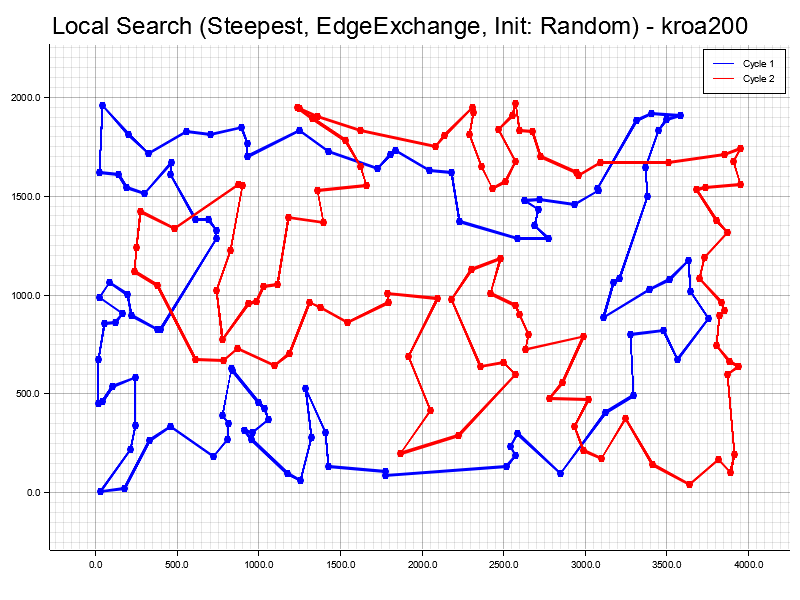
\includegraphics[width=\textwidth]{figures/kroa200_Local_Search_Steepest_EdgeExchange_Init_Random_.png}
        \caption{Instancja kroa200}
        \label{fig:steepest_kroa200}
    \end{subfigure}
    \hfill
    \begin{subfigure}[b]{0.6\textwidth}
        \centering
        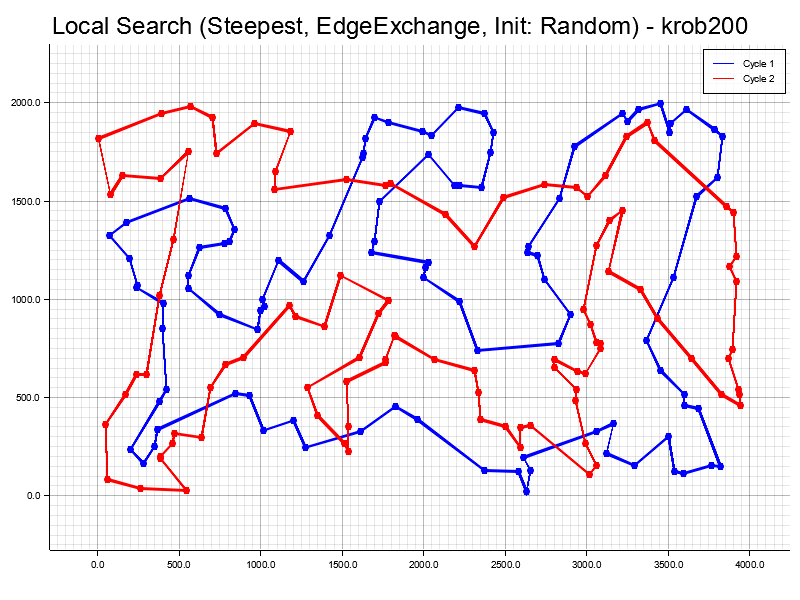
\includegraphics[width=\textwidth]{figures/krob200_Local_Search_Steepest_EdgeExchange_Init_Random_.png}
        \caption{Instancja krob200}
        \label{fig:steepest_krob200}
    \end{subfigure}
    \caption{Wizualizacje najlepszych rozwiązań dla LS Steepest (Random Init)}
    \label{fig:steepest}
\end{adjustwidth}
\end{figure}

\begin{figure}[H]
\begin{adjustwidth}{-1.5cm}{-1.5cm}
    \centering
    \begin{subfigure}[b]{0.6\textwidth}
        \centering
        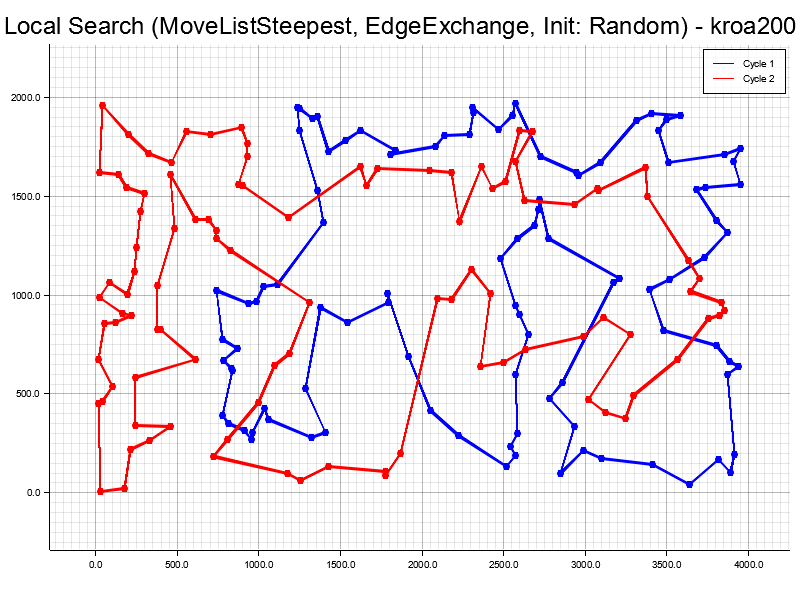
\includegraphics[width=\textwidth]{figures/kroa200_Local_Search_MoveListSteepest_EdgeExchange_Init_Random_.png}
        \caption{Instancja kroa200}
        \label{fig:movelist_kroa200}
    \end{subfigure}
    \hfill
    \begin{subfigure}[b]{0.6\textwidth}
        \centering
        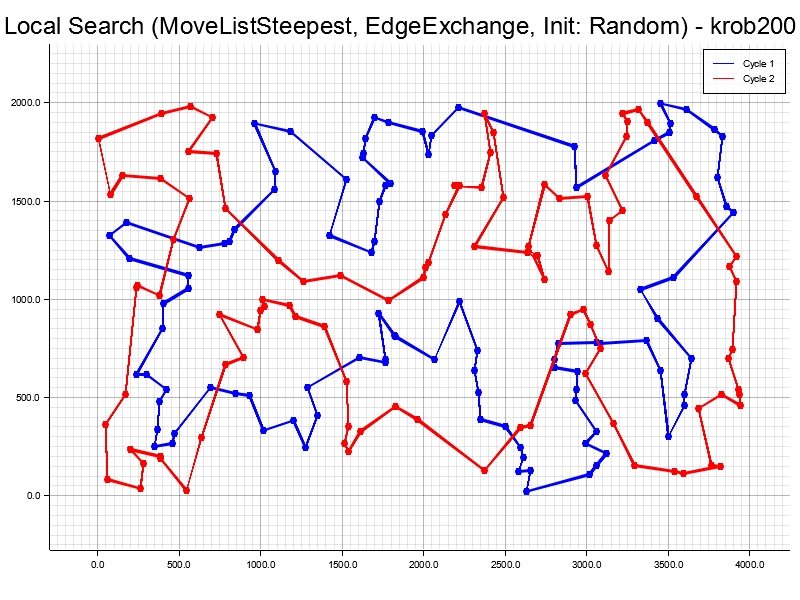
\includegraphics[width=\textwidth]{figures/krob200_Local_Search_MoveListSteepest_EdgeExchange_Init_Random_.png}
        \caption{Instancja krob200}
        \label{fig:movelist_krob200}
    \end{subfigure}
    \caption{Wizualizacje najlepszych rozwiązań dla LS Move List (Random Init)}
    \label{fig:movelist}
\end{adjustwidth}
\end{figure}

\begin{figure}[H]
\begin{adjustwidth}{-1.5cm}{-1.5cm}
    \centering
    \begin{subfigure}[b]{0.6\textwidth}
        \centering
        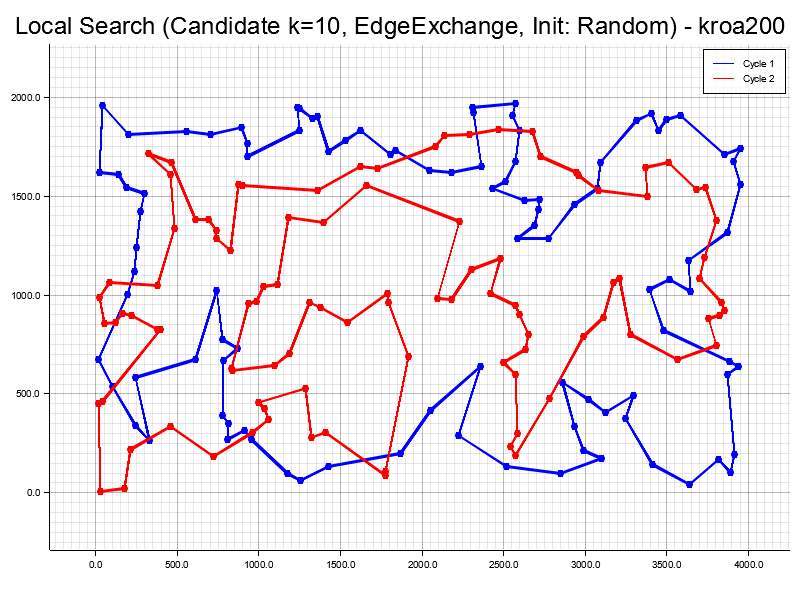
\includegraphics[width=\textwidth]{figures/kroa200_Local_Search_Candidate_k_10_EdgeExchange_Init_Random_.png}
        \caption{Instancja kroa200}
        \label{fig:candidate_kroa200}
    \end{subfigure}
    \hfill
    \begin{subfigure}[b]{0.6\textwidth}
        \centering
        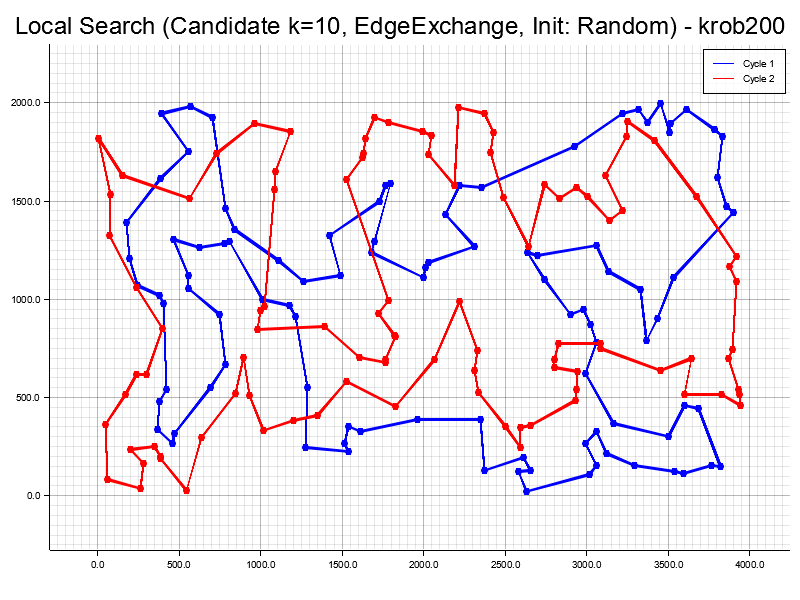
\includegraphics[width=\textwidth]{figures/krob200_Local_Search_Candidate_k_10_EdgeExchange_Init_Random_.png}
        \caption{Instancja krob200}
        \label{fig:candidate_krob200}
    \end{subfigure}
    \caption{Wizualizacje najlepszych rozwiązań dla LS Candidate k=10 (Random Init)}
    \label{fig:candidate}
\end{adjustwidth}
\end{figure}

\section{Wnioski}
Na podstawie przeprowadzonych eksperymentów z algorytmami przeszukiwania lokalnego startującymi z rozwiązań losowych można wyciągnąć następujące wnioski:

\begin{enumerate}
    \item \textbf{Jakość rozwiązań:} Najlepsze wyniki pod względem średniej jakości rozwiązania (najniższy średni koszt) nadal osiąga heurystyka konstrukcyjna \textbf{Ważony 2-żal} (średnio 36839 dla kroa200 i 37265 dla krob200), która dodatkowo znajduje lepsze rozwiązania minimalne niż algorytmy LS startujące z losowych rozwiązań. Spośród algorytmów przeszukiwania lokalnego, standardowy \textbf{LS Steepest} daje nieznacznie lepsze średnie wyniki (38348 / 38777) niż \textbf{LS Move List} (38894 / 38849), a oba te algorytmy są wyraźnie lepsze od \textbf{LS Candidate k=10} (40035 / 39735) pod względem średniego kosztu.

    \item \textbf{Czas wykonania:} Zgodnie z oczekiwaniami, usprawnienia mające na celu przyspieszenie LS działają. Najszybszy jest \textbf{LS Candidate k=10} (średnio 28 ms), który znacząco redukuje czas w porównaniu do standardowego \textbf{LS Steepest} (średnio 51 ms). Algorytm \textbf{LS Move List} również jest szybszy od wersji podstawowej (średnio 39 ms), co potwierdza skuteczność strategii aktualizacji listy ruchów zamiast pełnego przeszukiwania w każdej iteracji. Warto zauważyć, że heurystyka konstrukcyjna Ważony 2-żal jest najszybsza ze wszystkich (średnio 8.5 ms).

    \item \textbf{Kompromis jakość/czas:} \textbf{LS Candidate k=10} jest najszybszym wariantem LS, ale kosztem znaczącego pogorszenia jakości znajdowanych rozwiązań w porównaniu do LS Steepest i LS Move List. \textbf{LS Move List} oferuje dobry kompromis, będąc szybszym od LS Steepest przy jedynie minimalnym pogorszeniu (a w przypadku krob200 nawet nieznacznym polepszeniu) średniej jakości rozwiązania. \textbf{LS Steepest}, mimo że najwolniejszy z wariantów LS, daje średnio najlepsze wyniki jakościowe spośród nich.

    \item \textbf{Porównanie z heurystyką konstrukcyjną:} Żaden z testowanych wariantów przeszukiwania lokalnego, startujący z losowego rozwiązania, nie był w stanie średnio dorównać jakością ani szybkością najlepszej heurystyce konstrukcyjnej (Ważony 2-żal). Sugeruje to, że jakość rozwiązania początkowego ma duży wpływ na wynik końcowy LS, lub że zastosowane sąsiedztwo LS (wymiana krawędzi i wierzchołków) może nie być wystarczająco silne, aby znacząco poprawić losowe starty do poziomu rozwiązań konstrukcyjnych.

    \item \textbf{Wpływ strategii usprawnień:} Strategia listy ruchów (Move List) okazała się skuteczna w redukcji czasu przy niewielkim wpływie na jakość. Strategia ruchów kandydackich (Candidate k=10) znacząco przyspieszyła algorytm, ale kosztem zauważalnego spadku jakości. Dobór parametru `k` w metodzie Candidate może mieć istotny wpływ na ten kompromis.

\end{enumerate}

Podsumowując, usprawnienia algorytmu przeszukiwania lokalnego (Move List, Candidate Moves) pozwalają na skrócenie czasu jego działania. Wybór między nimi a wersją standardową zależy od priorytetu - szybkości czy jakości. Jednakże, w kontekście tego problemu i testowanych wariantów, wydaje się, że lepsze wyniki globalnie (zarówno pod względem jakości, jak i czasu) można uzyskać stosując zaawansowaną heurystykę konstrukcyjną, taką jak Ważony 2-żal, niż stosując przeszukiwanie lokalne na rozwiązaniach losowych.

\section{Kod źródłowy}
Pełny kod źródłowy implementacji wszystkich algorytmów jest dostępny w repozytorium GitHub:
\url{https://github.com/Veanir/imo-1}

\end{document} 